\documentclass{standalone}

\usepackage{amsmath}
\usepackage{tikz}
\usetikzlibrary{shapes, arrows.meta, positioning, backgrounds}

\tikzstyle{block} = [rectangle, minimum width=2cm, minimum height=1cm, text centered, draw=black, fill=white]
\tikzstyle{arrow} = [->,>=stealth]

\begin{document}
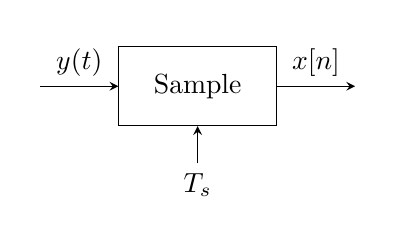
\begin{tikzpicture}[node distance=3cm, background rectangle/.style={fill=white}, show background rectangle]

    \node (block0) [block] at (0, 0) {Sample};
    \node (Ts0) at (0, -1.25) {$T_s$};

    \draw [arrow] (-2, 0) -- node[anchor=south] {$y(t)$} (block0);
    \draw [arrow] (block0) -- node[anchor=south] {$x[n]$} (2, 0);

    \draw [arrow] (Ts0) -- (block0);

\end{tikzpicture}
\end{document}